%  17 Apr 2025 11:39:09
\documentclass{article}
\usepackage{geometry,booktabs,longtable,pdflscape,rotating,threeparttable,subcaption,graphicx,float,}
\usepackage{tabularx,xcolor,colortbl,}
\usepackage{hyperref}
\hypersetup{                           colorlinks=true,                   linkcolor={blue!50!black},                    filecolor={blue!50!black},                 urlcolor={blue!80!black},                     }                              \date{}
\geometry{verbose,letterpaper,lmargin=2.5cm,tmargin=2.5cm}

\begin{document}

\title{Descriptives for Displacement Analysis Sample}
\maketitle
\section{Summary Table}
\begin{table}[htbp] 
\centering 
\begin{threeparttable} 
\caption{Summary Statistics by Displacement Status} 

\centering
\begin{tabular}{llll}
\toprule
\multicolumn{1}{c}{} &
  \multicolumn{1}{r}{All workers} &
  \multicolumn{1}{r}{Non-Displaced} &
  \multicolumn{1}{r}{Displaced} \\
\midrule
\multicolumn{1}{l}{Birth Year} &
  \multicolumn{1}{c}{1956.7} &
  \multicolumn{1}{c}{1956.7} &
  \multicolumn{1}{c}{1956.7} \\
\multicolumn{1}{l}{} &
  \multicolumn{1}{c}{[9.2]} &
  \multicolumn{1}{c}{[9.2]} &
  \multicolumn{1}{c}{[9.2]} \\
\multicolumn{1}{l}{Age} &
  \multicolumn{1}{c}{41.0} &
  \multicolumn{1}{c}{41.0} &
  \multicolumn{1}{c}{41.0} \\
\multicolumn{1}{l}{} &
  \multicolumn{1}{c}{[8.3]} &
  \multicolumn{1}{c}{[8.3]} &
  \multicolumn{1}{c}{[8.3]} \\
\multicolumn{1}{l}{Female} &
  \multicolumn{1}{c}{0.3} &
  \multicolumn{1}{c}{0.3} &
  \multicolumn{1}{c}{0.3} \\
\multicolumn{1}{l}{} &
  \multicolumn{1}{c}{[0.5]} &
  \multicolumn{1}{c}{[0.5]} &
  \multicolumn{1}{c}{[0.5]} \\
\multicolumn{1}{l}{Years of Schooling} &
  \multicolumn{1}{c}{11.6} &
  \multicolumn{1}{c}{11.6} &
  \multicolumn{1}{c}{11.6} \\
\multicolumn{1}{l}{} &
  \multicolumn{1}{c}{[2.3]} &
  \multicolumn{1}{c}{[2.3]} &
  \multicolumn{1}{c}{[2.3]} \\
\multicolumn{1}{l}{Earnings} &
  \multicolumn{1}{c}{11943.3} &
  \multicolumn{1}{c}{11943.3} &
  \multicolumn{1}{c}{11943.3} \\
\multicolumn{1}{l}{} &
  \multicolumn{1}{c}{[3350.4]} &
  \multicolumn{1}{c}{[3350.4]} &
  \multicolumn{1}{c}{[3350.4]} \\
\multicolumn{1}{l}{Log Earnings} &
  \multicolumn{1}{c}{9.4} &
  \multicolumn{1}{c}{9.4} &
  \multicolumn{1}{c}{9.4} \\
\multicolumn{1}{l}{} &
  \multicolumn{1}{c}{[0.3]} &
  \multicolumn{1}{c}{[0.3]} &
  \multicolumn{1}{c}{[0.3]} \\
\multicolumn{1}{l}{Employed} &
  \multicolumn{1}{c}{1.0} &
  \multicolumn{1}{c}{1.0} &
  \multicolumn{1}{c}{1.0} \\
\multicolumn{1}{l}{} &
  \multicolumn{1}{c}{[0.0]} &
  \multicolumn{1}{c}{[0.0]} &
  \multicolumn{1}{c}{[0.0]} \\
\multicolumn{1}{l}{Firm size} &
  \multicolumn{1}{c}{512.3} &
  \multicolumn{1}{c}{512.3} &
  \multicolumn{1}{c}{512.3} \\
\multicolumn{1}{l}{} &
  \multicolumn{1}{c}{[454.8]} &
  \multicolumn{1}{c}{[454.8]} &
  \multicolumn{1}{c}{[454.8]} \\
\midrule
\multicolumn{1}{l}{Number of Observations} &
  \multicolumn{1}{c}{394} &
  \multicolumn{1}{c}{394} &
  \multicolumn{1}{c}{394} \\
\multicolumn{1}{l}{Number of Establishments} &
  \multicolumn{1}{c}{91} &
  \multicolumn{1}{c}{83} &
  \multicolumn{1}{c}{86} \\
\bottomrule
\end{tabular}

 \footnotesize  
\textbf{Notes:} Average characteristics of individuals. Standard deviations in brackets. 
\end{threeparttable} 
\end{table}
\begin{table}[htbp] 
\centering 
\begin{threeparttable} 
\caption{Summary Statistics with Percentiles} 

\centering
\begin{tabular}{lllllllll}
\toprule
\multicolumn{1}{c}{} &
  \multicolumn{1}{c}{10th pct} &
  \multicolumn{1}{c}{25th pct} &
  \multicolumn{1}{c}{50th pct} &
  \multicolumn{1}{c}{75th pct} &
  \multicolumn{1}{c}{90th pct} &
  \multicolumn{1}{c}{Mean} &
  \multicolumn{1}{c}{SD} &
  \multicolumn{1}{c}{N} \\
\midrule
\multicolumn{1}{l}{Birth Year} &
  \multicolumn{1}{c}{1943.00} &
  \multicolumn{1}{c}{1950.00} &
  \multicolumn{1}{c}{1956.00} &
  \multicolumn{1}{c}{1964.00} &
  \multicolumn{1}{c}{1970.00} &
  \multicolumn{1}{c}{1956.68} &
  \multicolumn{1}{c}{[9.20]} &
  \multicolumn{1}{c}{394} \\
\multicolumn{1}{l}{Age} &
  \multicolumn{1}{c}{30.00} &
  \multicolumn{1}{c}{34.00} &
  \multicolumn{1}{c}{40.00} &
  \multicolumn{1}{c}{48.00} &
  \multicolumn{1}{c}{53.00} &
  \multicolumn{1}{c}{41.04} &
  \multicolumn{1}{c}{[8.26]} &
  \multicolumn{1}{c}{394} \\
\multicolumn{1}{l}{Female} &
  \multicolumn{1}{c}{0.00} &
  \multicolumn{1}{c}{0.00} &
  \multicolumn{1}{c}{0.00} &
  \multicolumn{1}{c}{1.00} &
  \multicolumn{1}{c}{1.00} &
  \multicolumn{1}{c}{0.31} &
  \multicolumn{1}{c}{[0.46]} &
  \multicolumn{1}{c}{394} \\
\multicolumn{1}{l}{Years of Schooling} &
  \multicolumn{1}{c}{8.00} &
  \multicolumn{1}{c}{10.00} &
  \multicolumn{1}{c}{12.00} &
  \multicolumn{1}{c}{14.00} &
  \multicolumn{1}{c}{15.00} &
  \multicolumn{1}{c}{11.63} &
  \multicolumn{1}{c}{[2.29]} &
  \multicolumn{1}{c}{394} \\
\multicolumn{1}{l}{Earnings} &
  \multicolumn{1}{c}{8087.93} &
  \multicolumn{1}{c}{9416.35} &
  \multicolumn{1}{c}{11417.13} &
  \multicolumn{1}{c}{14096.48} &
  \multicolumn{1}{c}{16701.68} &
  \multicolumn{1}{c}{11943.30} &
  \multicolumn{1}{c}{[3350.41]} &
  \multicolumn{1}{c}{394} \\
\multicolumn{1}{l}{Log Earnings} &
  \multicolumn{1}{c}{9.00} &
  \multicolumn{1}{c}{9.15} &
  \multicolumn{1}{c}{9.34} &
  \multicolumn{1}{c}{9.55} &
  \multicolumn{1}{c}{9.72} &
  \multicolumn{1}{c}{9.35} &
  \multicolumn{1}{c}{[0.27]} &
  \multicolumn{1}{c}{394} \\
\multicolumn{1}{l}{Employed} &
  \multicolumn{1}{c}{1.00} &
  \multicolumn{1}{c}{1.00} &
  \multicolumn{1}{c}{1.00} &
  \multicolumn{1}{c}{1.00} &
  \multicolumn{1}{c}{1.00} &
  \multicolumn{1}{c}{1.00} &
  \multicolumn{1}{c}{[0.00]} &
  \multicolumn{1}{c}{394} \\
\multicolumn{1}{l}{Firm size} &
  \multicolumn{1}{c}{115.81} &
  \multicolumn{1}{c}{188.56} &
  \multicolumn{1}{c}{366.99} &
  \multicolumn{1}{c}{629.32} &
  \multicolumn{1}{c}{1099.06} &
  \multicolumn{1}{c}{512.35} &
  \multicolumn{1}{c}{[454.78]} &
  \multicolumn{1}{c}{394} \\
\bottomrule
\end{tabular}

\end{threeparttable} 
\end{table}
\begin{table}[htbp] 
\centering 
\begin{threeparttable} 
\caption{Industry Distribution by Displacement Status} 

\centering
\begin{tabular}{lll}
\toprule
\multicolumn{1}{c}{} &
  \multicolumn{1}{c}{Non-displaced} &
  \multicolumn{1}{c}{Displaced} \\
\midrule
\multicolumn{1}{c}{Mining} &
  \multicolumn{1}{c}{13.7} &
  \multicolumn{1}{c}{13.7} \\
\multicolumn{1}{c}{Construction} &
  \multicolumn{1}{c}{11.7} &
  \multicolumn{1}{c}{11.7} \\
\multicolumn{1}{c}{Manufacturing} &
  \multicolumn{1}{c}{16.8} &
  \multicolumn{1}{c}{16.8} \\
\multicolumn{1}{c}{Health} &
  \multicolumn{1}{c}{11.2} &
  \multicolumn{1}{c}{11.2} \\
\multicolumn{1}{c}{Finance} &
  \multicolumn{1}{c}{17.8} &
  \multicolumn{1}{c}{17.8} \\
\multicolumn{1}{c}{FCSL} &
  \multicolumn{1}{c}{19.3} &
  \multicolumn{1}{c}{19.3} \\
\multicolumn{1}{c}{Professional Services} &
  \multicolumn{1}{c}{9.6} &
  \multicolumn{1}{c}{9.6} \\
\multicolumn{1}{c}{Total} &
  \multicolumn{1}{c}{100.0} &
  \multicolumn{1}{c}{100.0} \\
\bottomrule
\end{tabular}

\end{threeparttable} 
\end{table}
\begin{table}[htbp] 
\centering 
\begin{threeparttable} 
\caption{Number of Workers by Industry and Year} 

\centering
\begin{tabular}{lllllllllll}
\toprule
\multicolumn{1}{c}{} &
  \multicolumn{1}{r}{1993} &
  \multicolumn{1}{r}{1994} &
  \multicolumn{1}{r}{1995} &
  \multicolumn{1}{r}{1996} &
  \multicolumn{1}{r}{1997} &
  \multicolumn{1}{r}{2000} &
  \multicolumn{1}{r}{2001} &
  \multicolumn{1}{r}{2002} &
  \multicolumn{1}{r}{2003} &
  \multicolumn{1}{r}{2004} \\
\midrule
\multicolumn{1}{l}{Mining} &
  \multicolumn{1}{r}{2} &
  \multicolumn{1}{r}{2} &
  \multicolumn{1}{r}{14} &
  \multicolumn{1}{r}{6} &
  \multicolumn{1}{r}{8} &
  \multicolumn{1}{r}{6} &
  \multicolumn{1}{r}{6} &
  \multicolumn{1}{r}{8} &
  \multicolumn{1}{r}{2} &
  \multicolumn{1}{r}{} \\
\multicolumn{1}{l}{Construction} &
  \multicolumn{1}{r}{6} &
  \multicolumn{1}{r}{10} &
  \multicolumn{1}{r}{6} &
  \multicolumn{1}{r}{} &
  \multicolumn{1}{r}{} &
  \multicolumn{1}{r}{6} &
  \multicolumn{1}{r}{10} &
  \multicolumn{1}{r}{8} &
  \multicolumn{1}{r}{} &
  \multicolumn{1}{r}{} \\
\multicolumn{1}{l}{Manufacturing} &
  \multicolumn{1}{r}{16} &
  \multicolumn{1}{r}{2} &
  \multicolumn{1}{r}{14} &
  \multicolumn{1}{r}{4} &
  \multicolumn{1}{r}{6} &
  \multicolumn{1}{r}{8} &
  \multicolumn{1}{r}{6} &
  \multicolumn{1}{r}{2} &
  \multicolumn{1}{r}{4} &
  \multicolumn{1}{r}{4} \\
\multicolumn{1}{l}{Health} &
  \multicolumn{1}{r}{12} &
  \multicolumn{1}{r}{} &
  \multicolumn{1}{r}{8} &
  \multicolumn{1}{r}{2} &
  \multicolumn{1}{r}{6} &
  \multicolumn{1}{r}{4} &
  \multicolumn{1}{r}{12} &
  \multicolumn{1}{r}{} &
  \multicolumn{1}{r}{} &
  \multicolumn{1}{r}{} \\
\multicolumn{1}{l}{Finance} &
  \multicolumn{1}{r}{8} &
  \multicolumn{1}{r}{12} &
  \multicolumn{1}{r}{18} &
  \multicolumn{1}{r}{} &
  \multicolumn{1}{r}{8} &
  \multicolumn{1}{r}{4} &
  \multicolumn{1}{r}{4} &
  \multicolumn{1}{r}{4} &
  \multicolumn{1}{r}{8} &
  \multicolumn{1}{r}{4} \\
\multicolumn{1}{l}{FCSL} &
  \multicolumn{1}{r}{8} &
  \multicolumn{1}{r}{8} &
  \multicolumn{1}{r}{4} &
  \multicolumn{1}{r}{4} &
  \multicolumn{1}{r}{4} &
  \multicolumn{1}{r}{4} &
  \multicolumn{1}{r}{4} &
  \multicolumn{1}{r}{22} &
  \multicolumn{1}{r}{10} &
  \multicolumn{1}{r}{8} \\
\multicolumn{1}{l}{Professional Services} &
  \multicolumn{1}{r}{8} &
  \multicolumn{1}{r}{6} &
  \multicolumn{1}{r}{} &
  \multicolumn{1}{r}{8} &
  \multicolumn{1}{r}{4} &
  \multicolumn{1}{r}{} &
  \multicolumn{1}{r}{8} &
  \multicolumn{1}{r}{} &
  \multicolumn{1}{r}{4} &
  \multicolumn{1}{r}{} \\
\bottomrule
\end{tabular}

 \footnotesize  
\textbf{Notes:} Each cell shows number of workers per cell 
\end{threeparttable} 
\end{table}
\section{Consistency Checks}
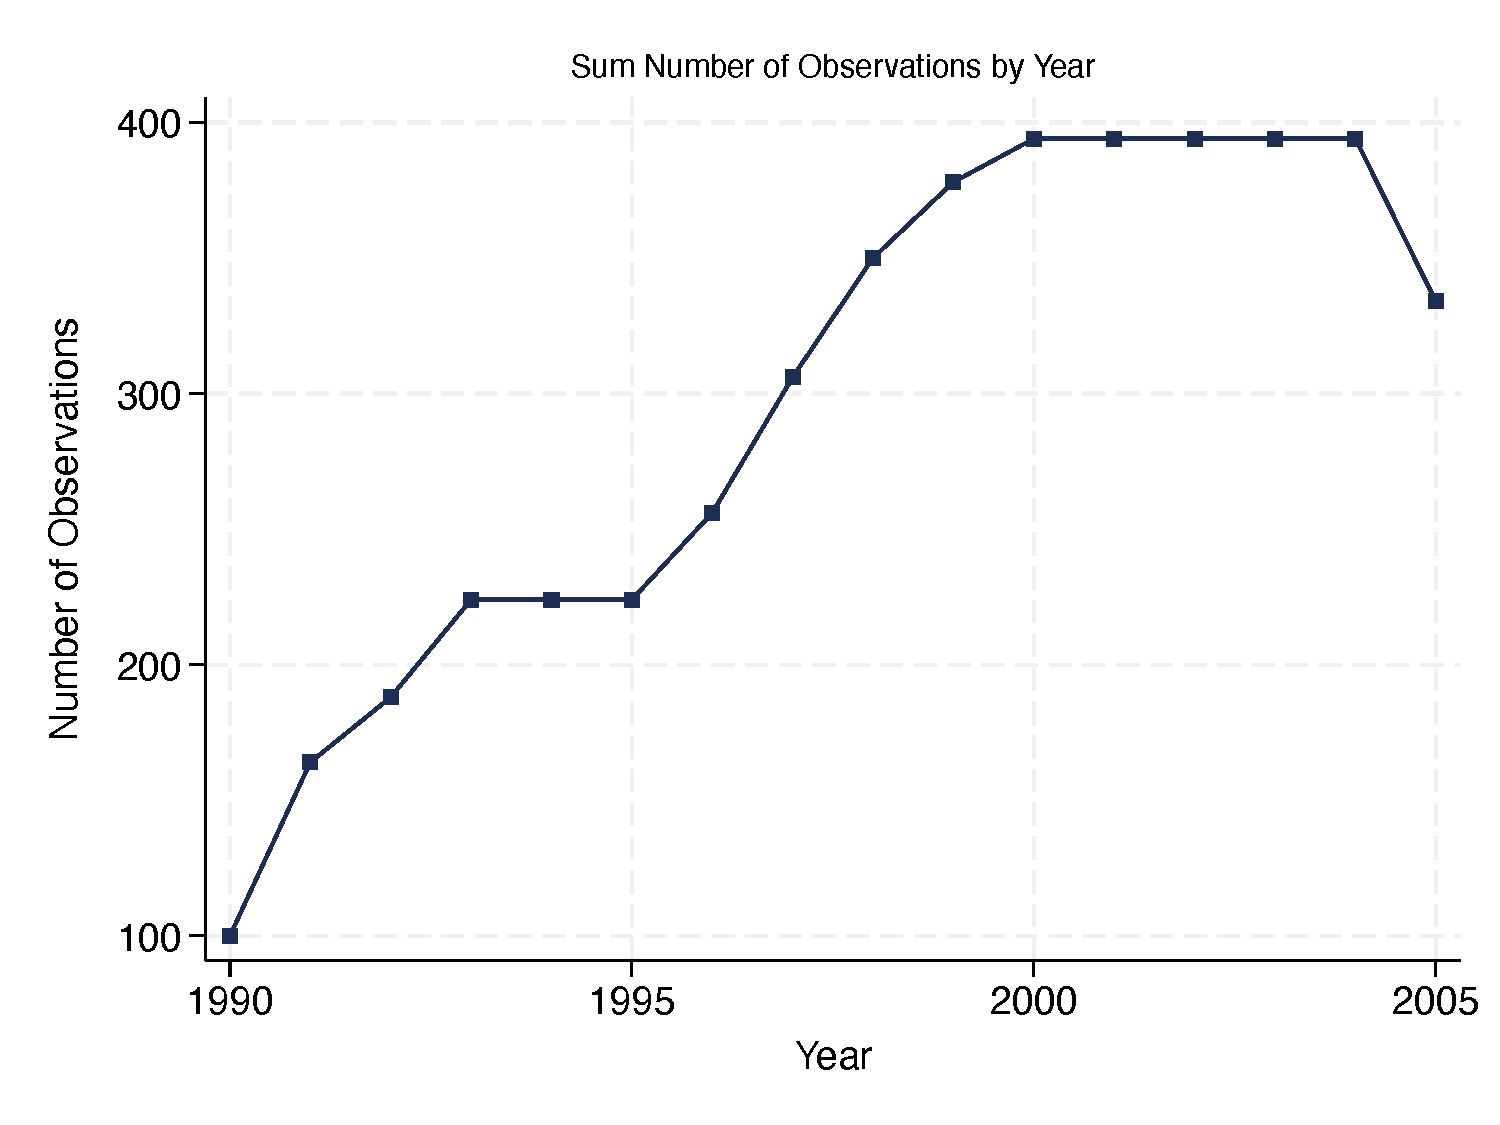
\includegraphics[width = .9\textwidth]{Consistency/counts_by_time.pdf} \\ 
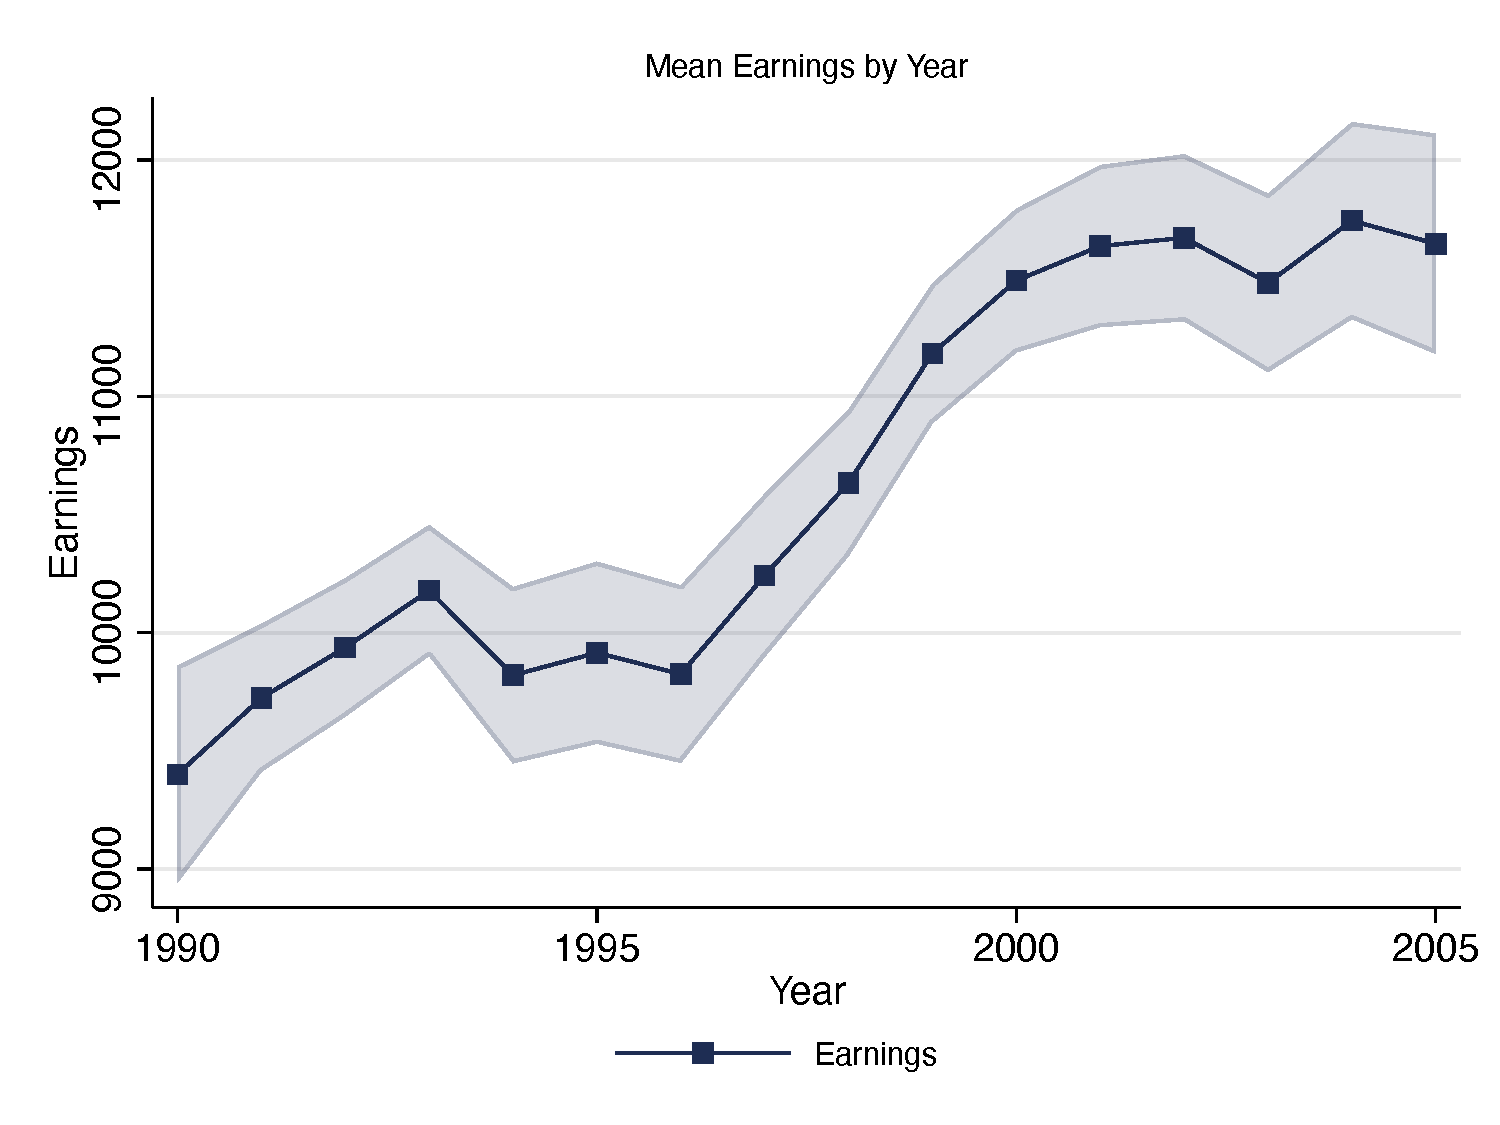
\includegraphics[width = .9\textwidth]{Consistency/earn_by_time.pdf} \\ 
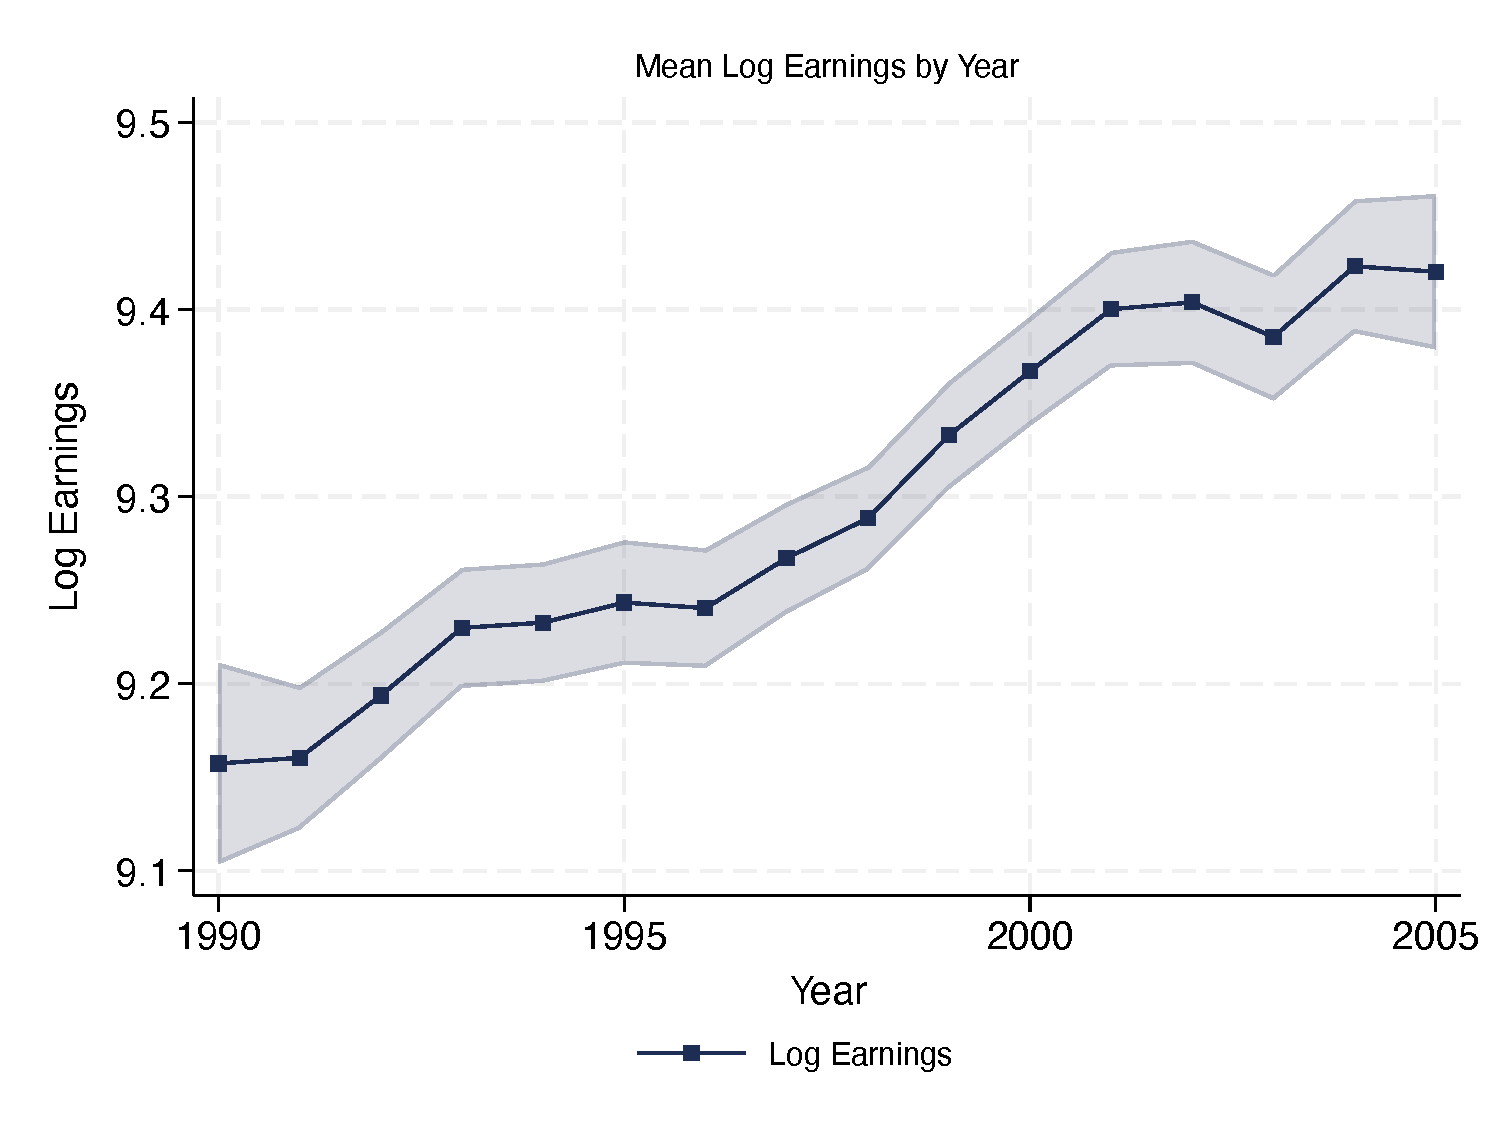
\includegraphics[width = .9\textwidth]{Consistency/logearn_by_time.pdf} \\ 
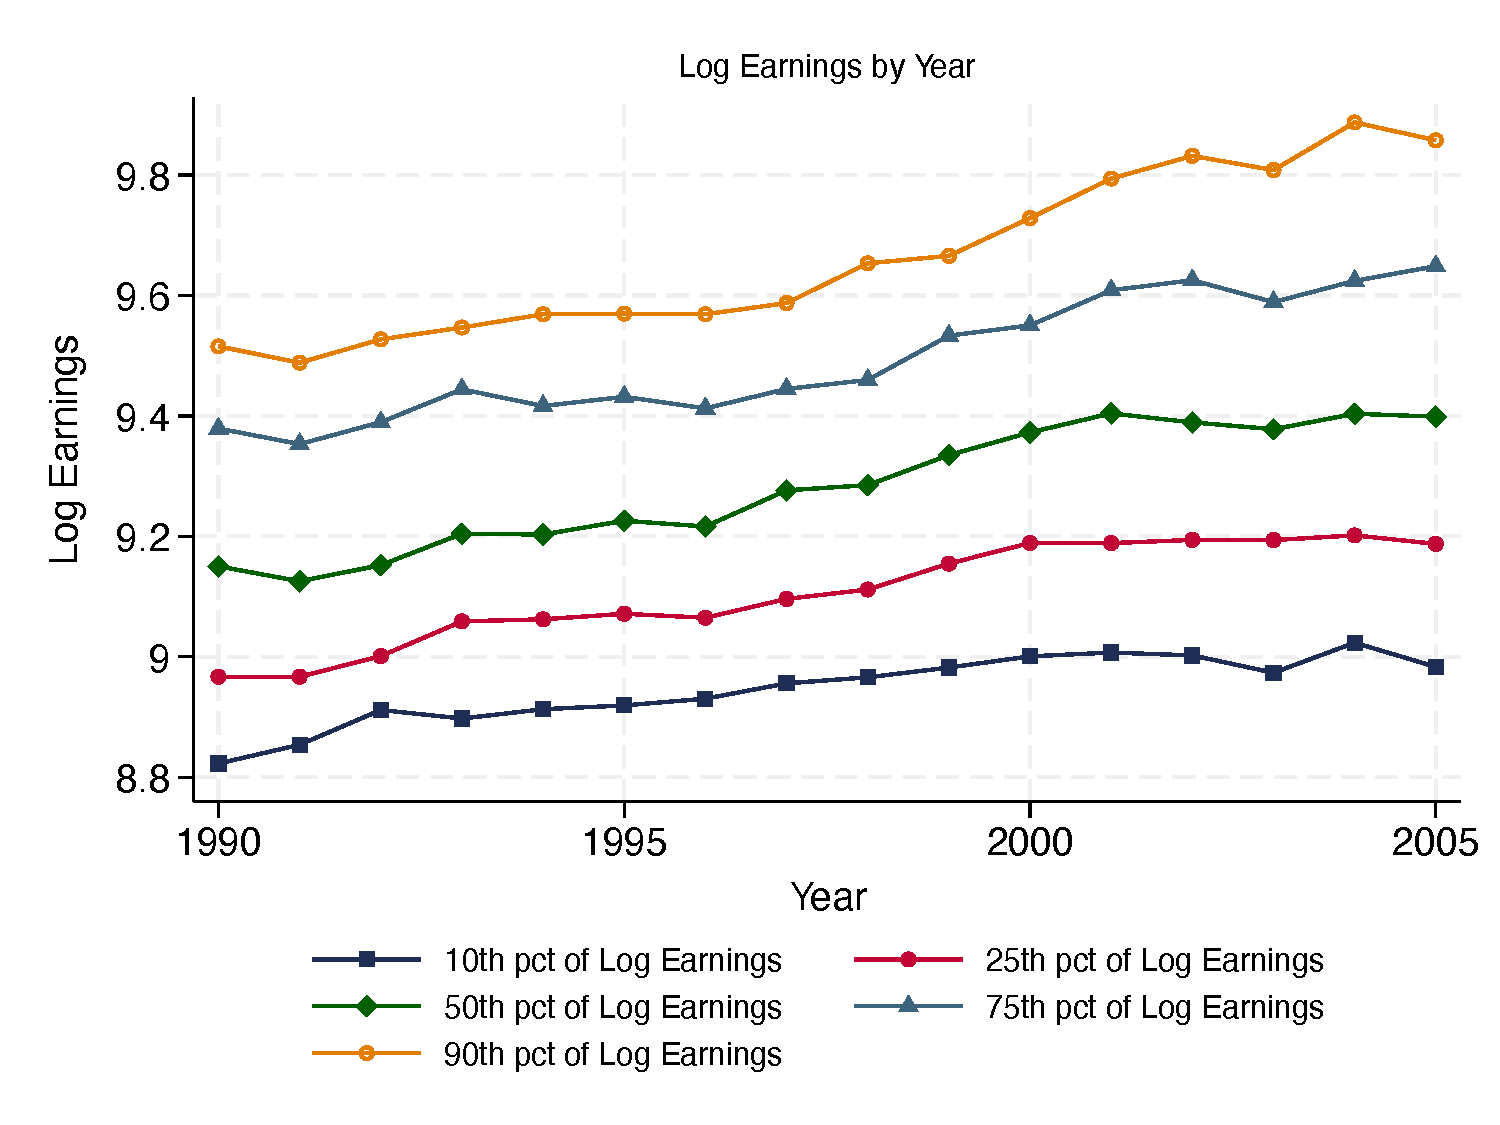
\includegraphics[width = .9\textwidth]{Consistency/logearn_by_year_pct.pdf} \\ 
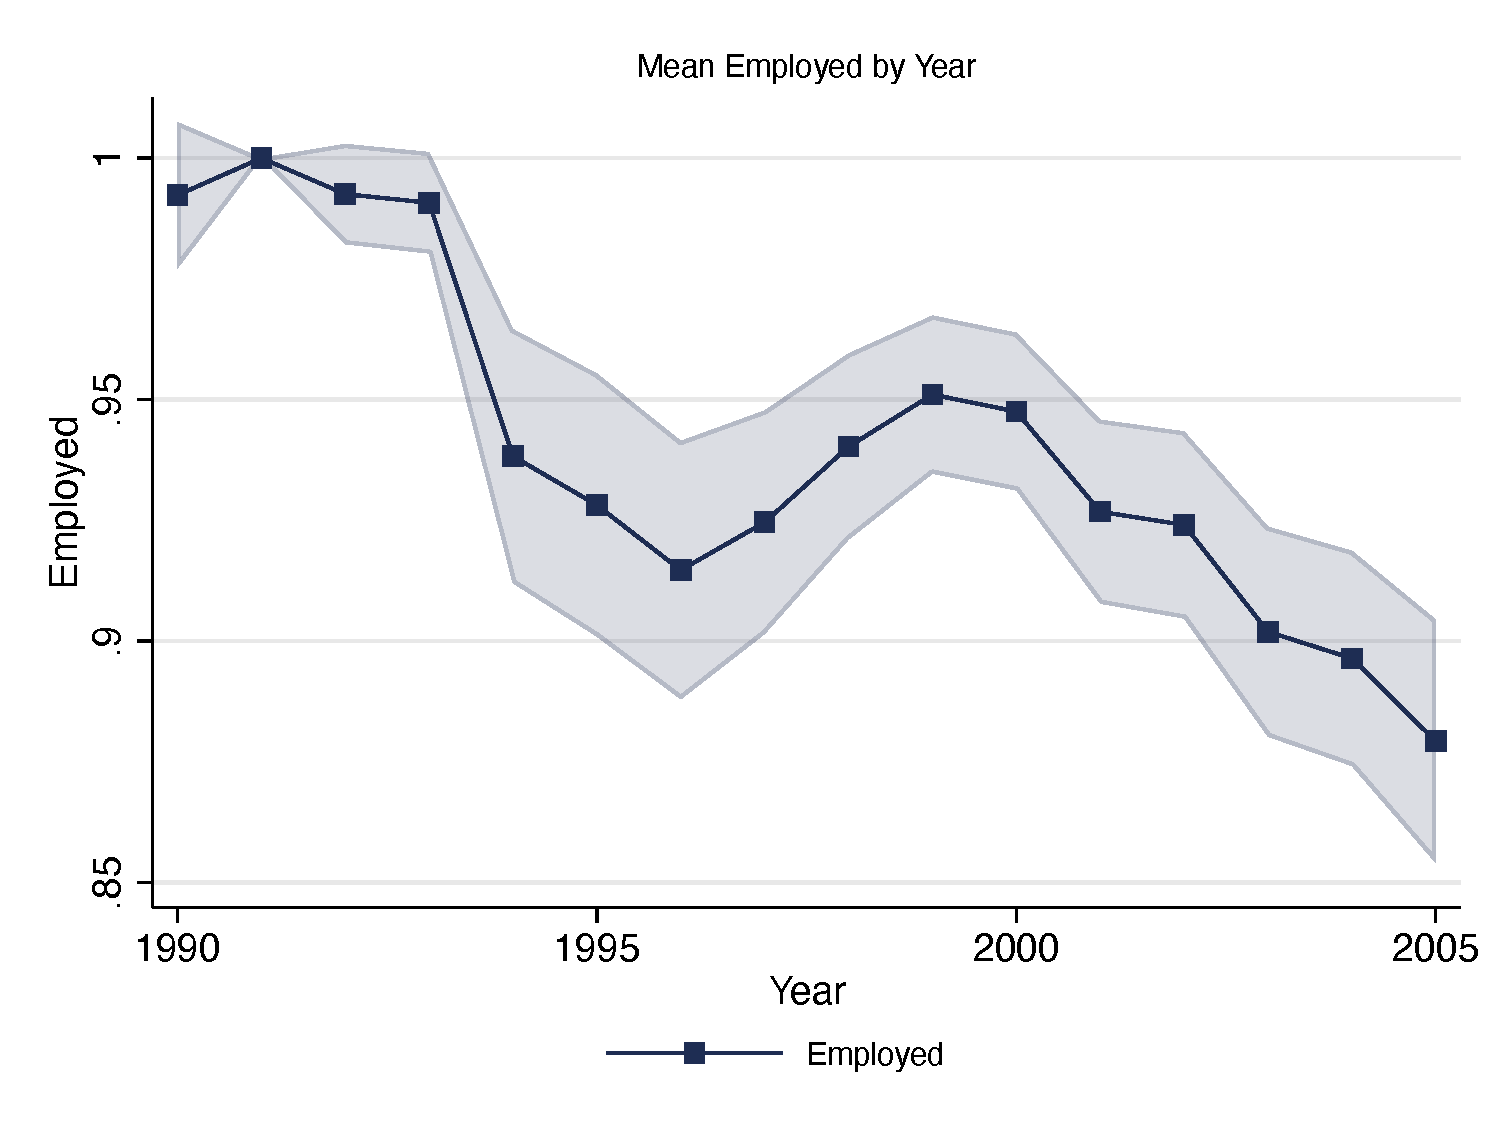
\includegraphics[width = .9\textwidth]{Consistency/employed_by_time.pdf} \\ 
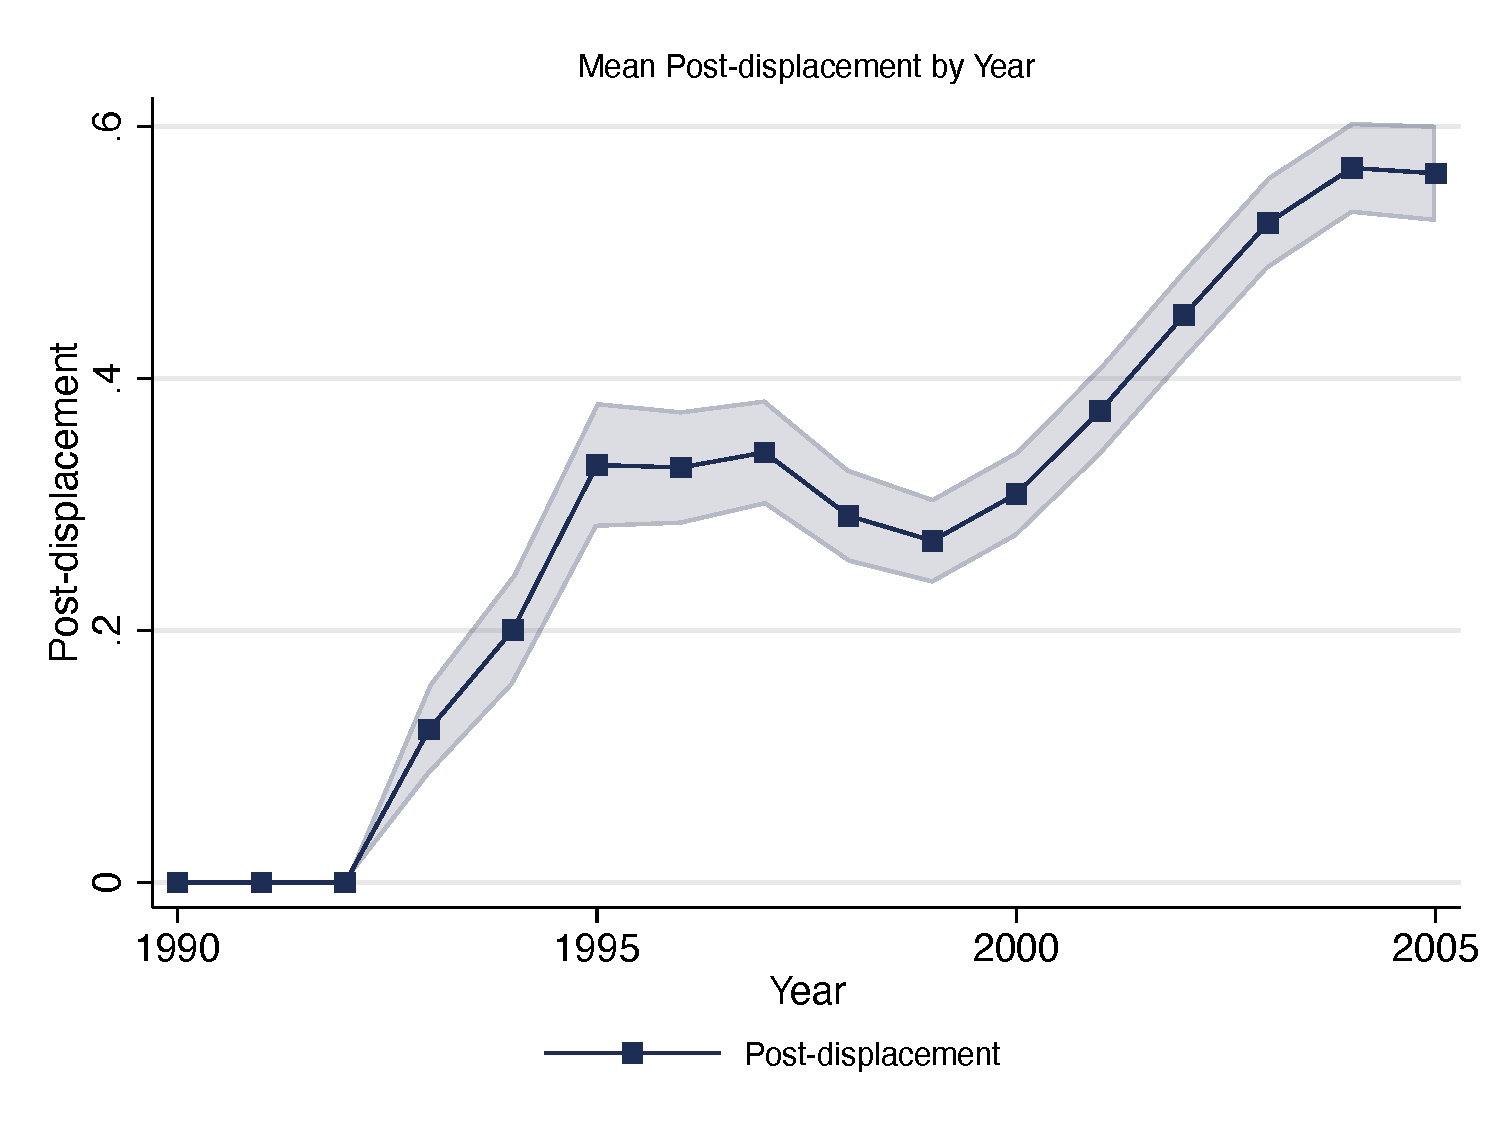
\includegraphics[width = .9\textwidth]{Consistency/displaced_by_time.pdf} \\ 
\section{Treatment and Control around Displacement Event}
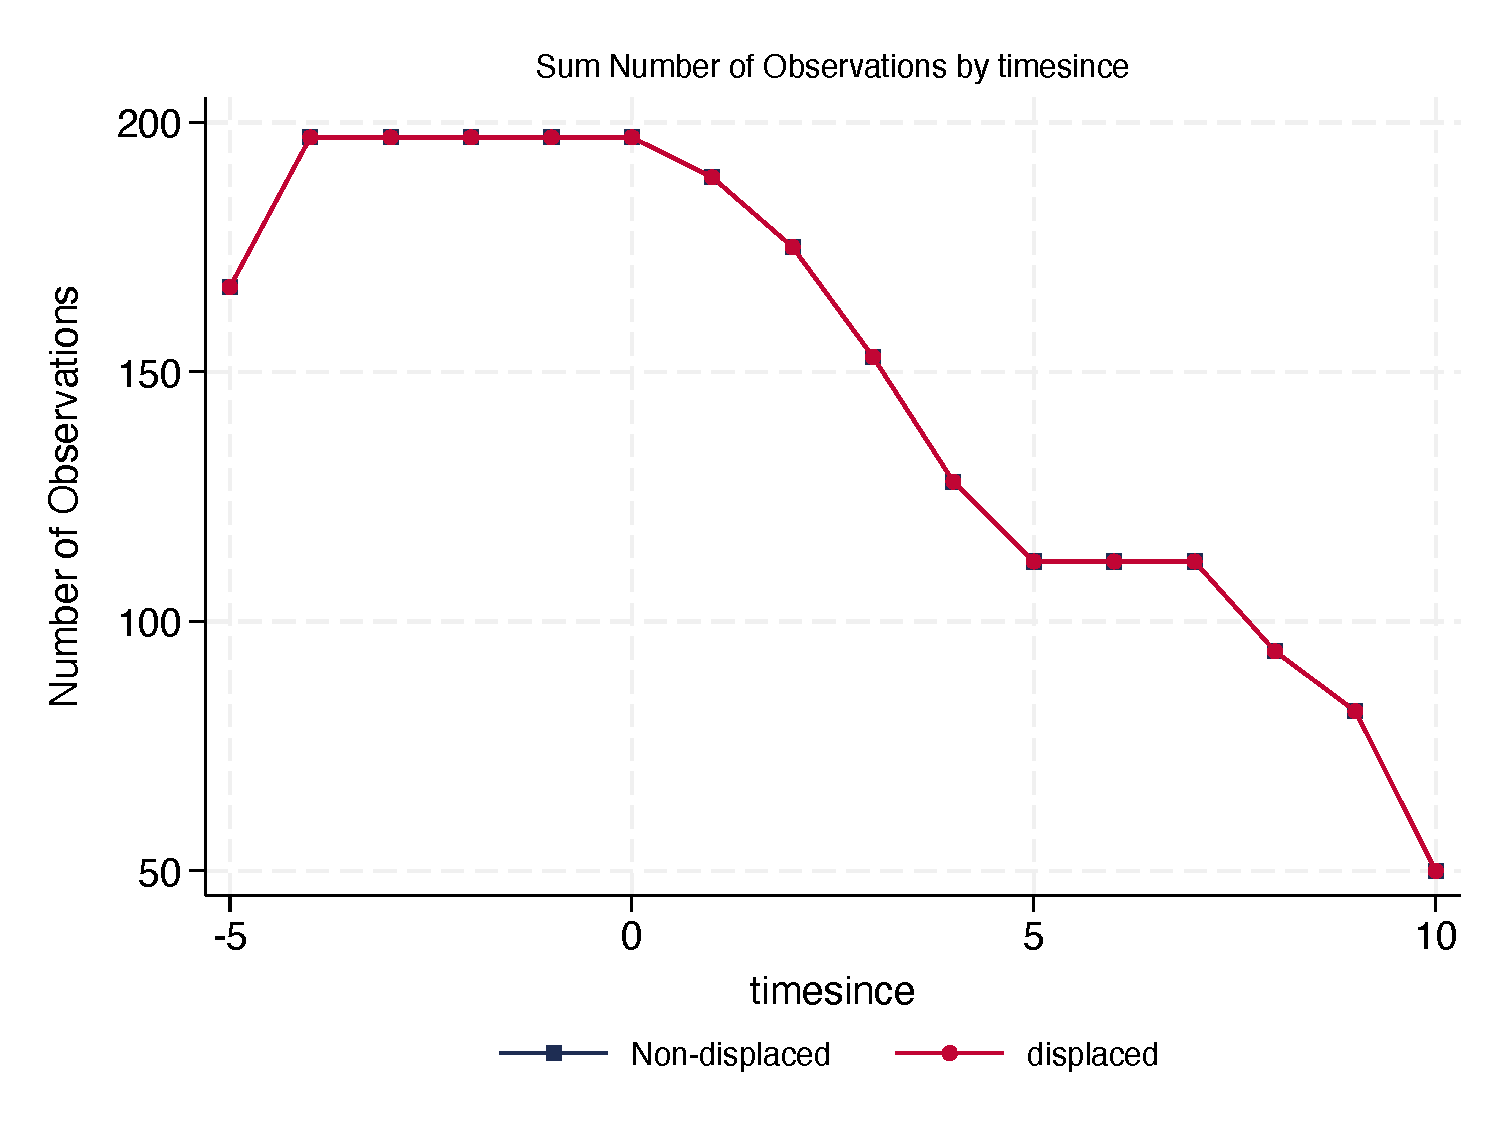
\includegraphics[width = .9\textwidth]{Disp_event_raw/counts_by_timesince.pdf} \\ 
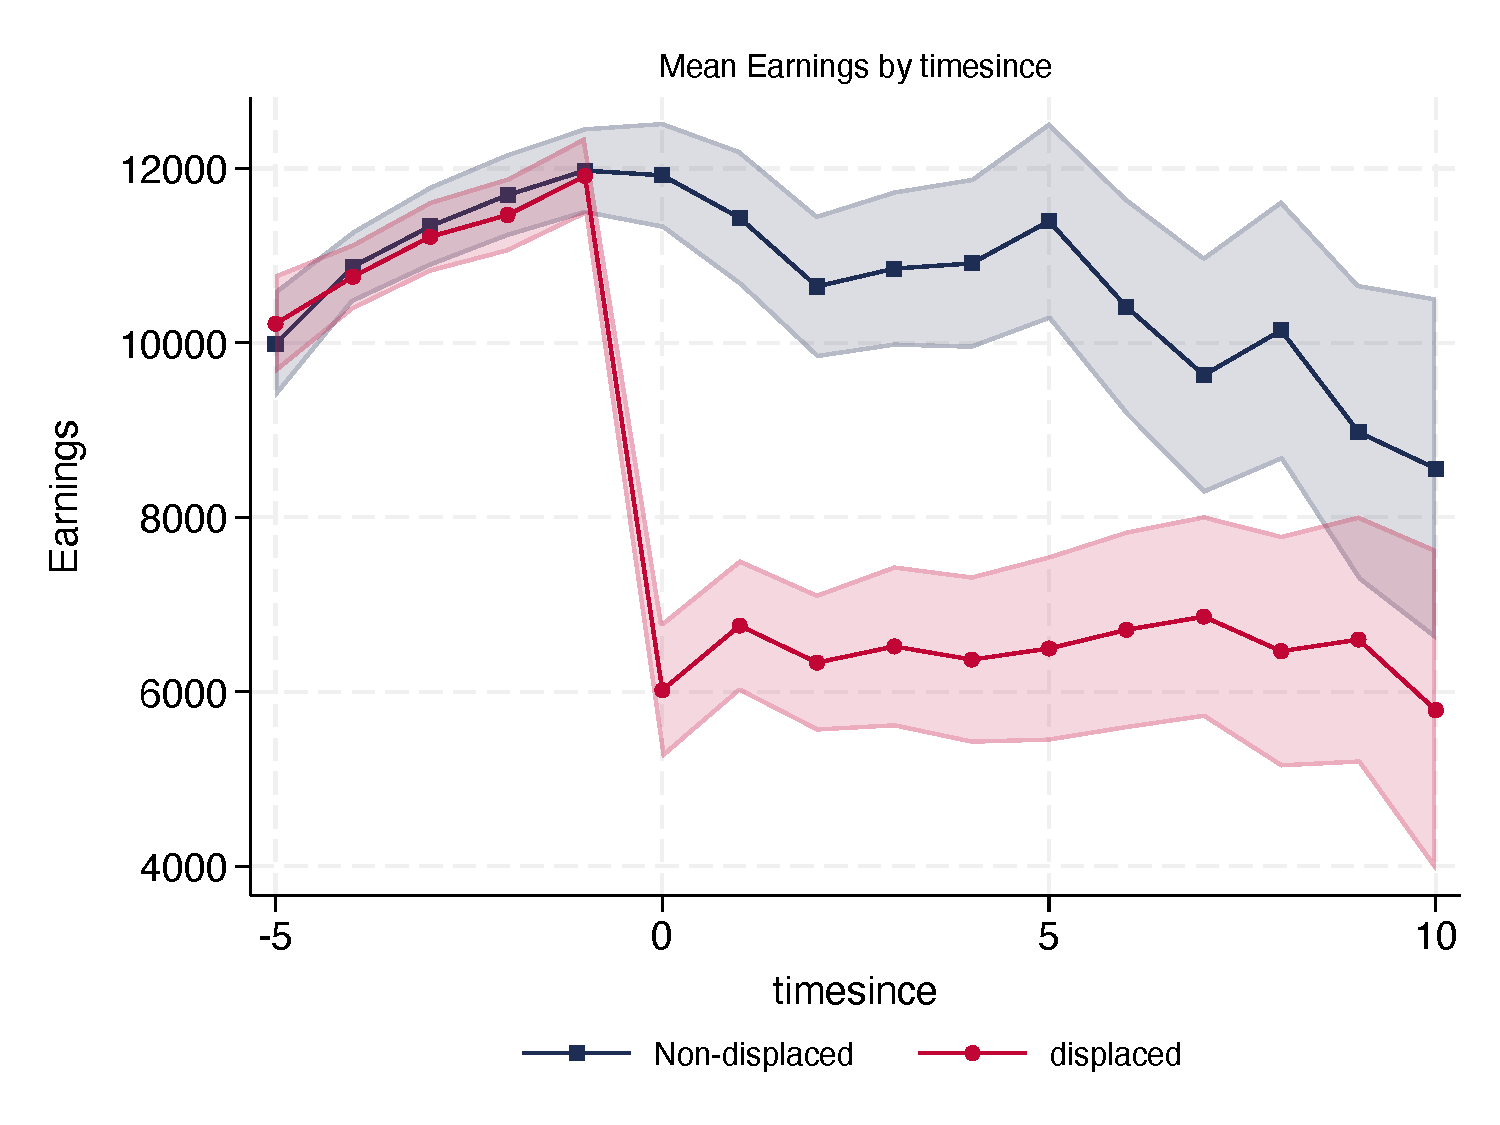
\includegraphics[width = .9\textwidth]{Disp_event_raw/logearn_by_timesince.pdf} \\ 
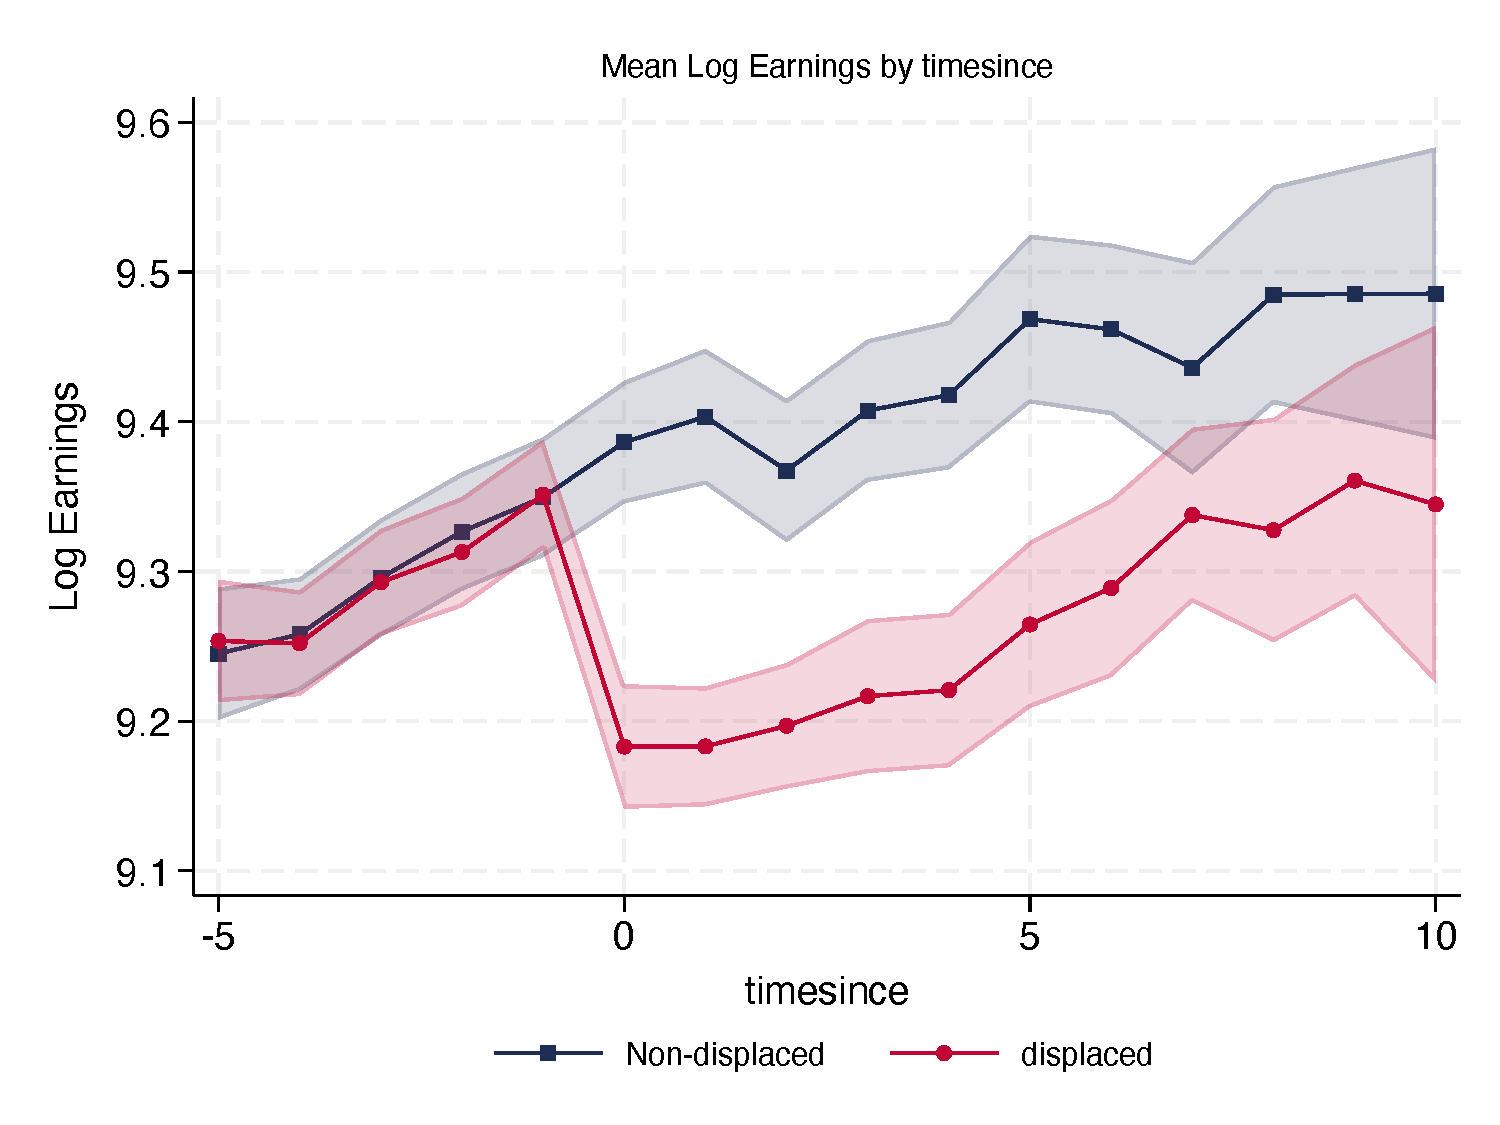
\includegraphics[width = .9\textwidth]{Disp_event_raw/earn_by_timesince.pdf} \\ 
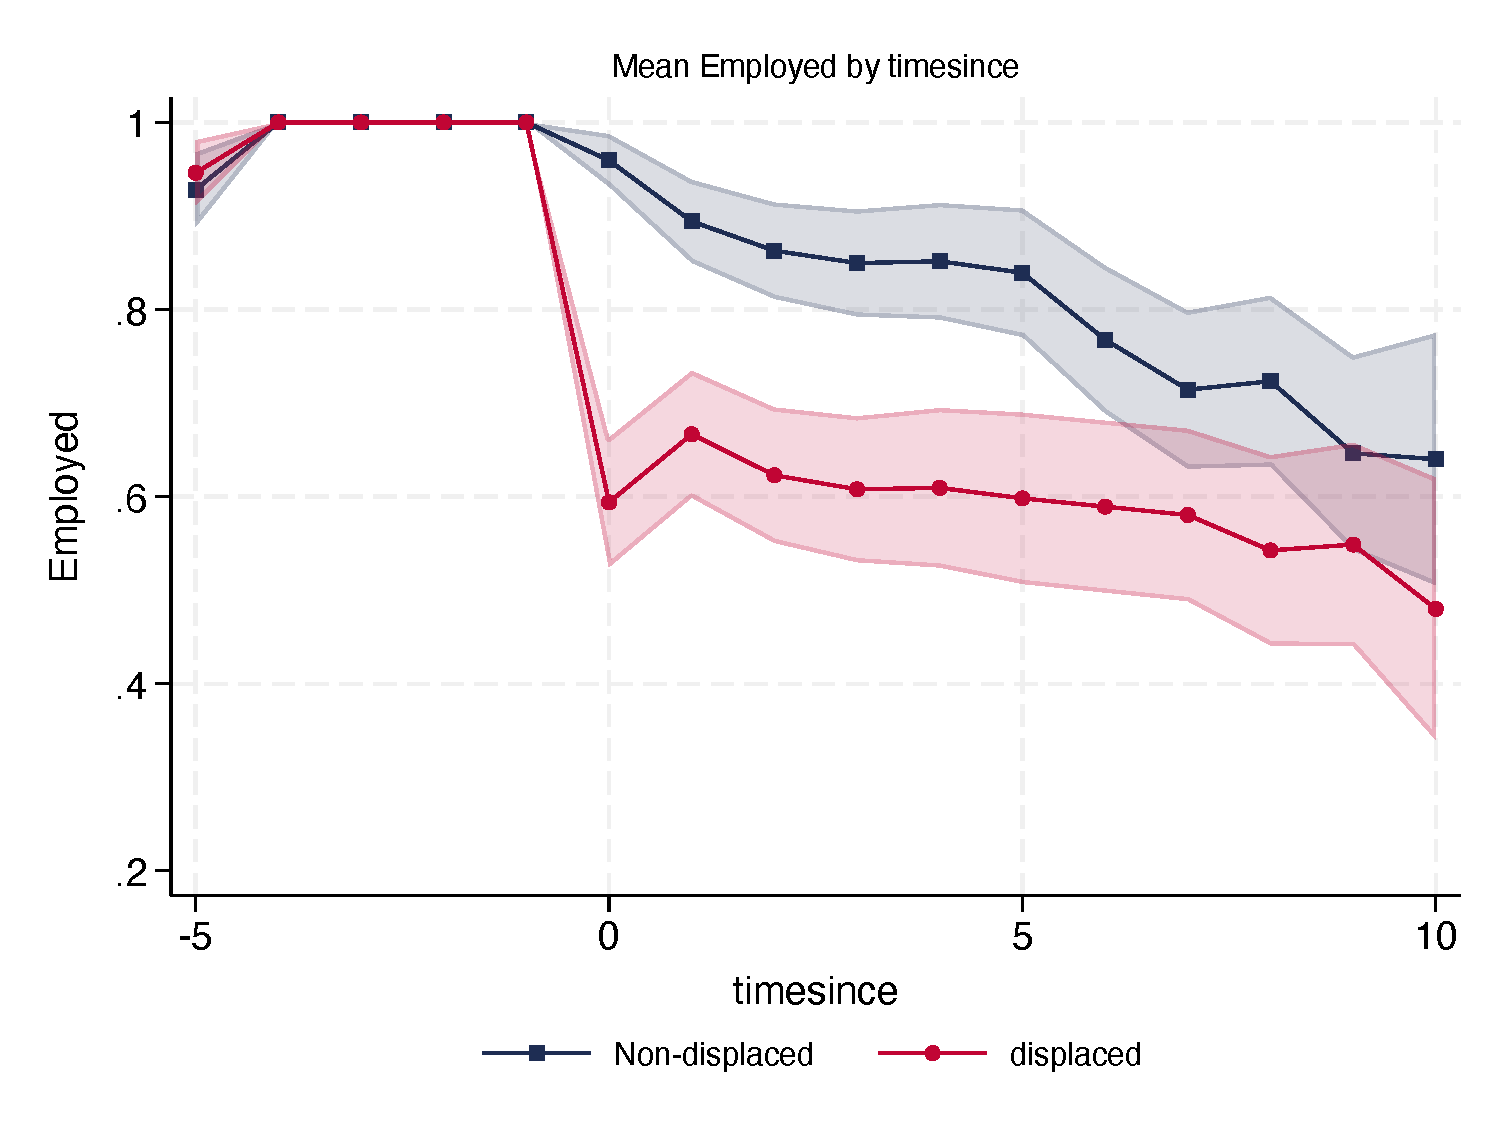
\includegraphics[width = .9\textwidth]{Disp_event_raw/employed_by_timesince.pdf} \\ 
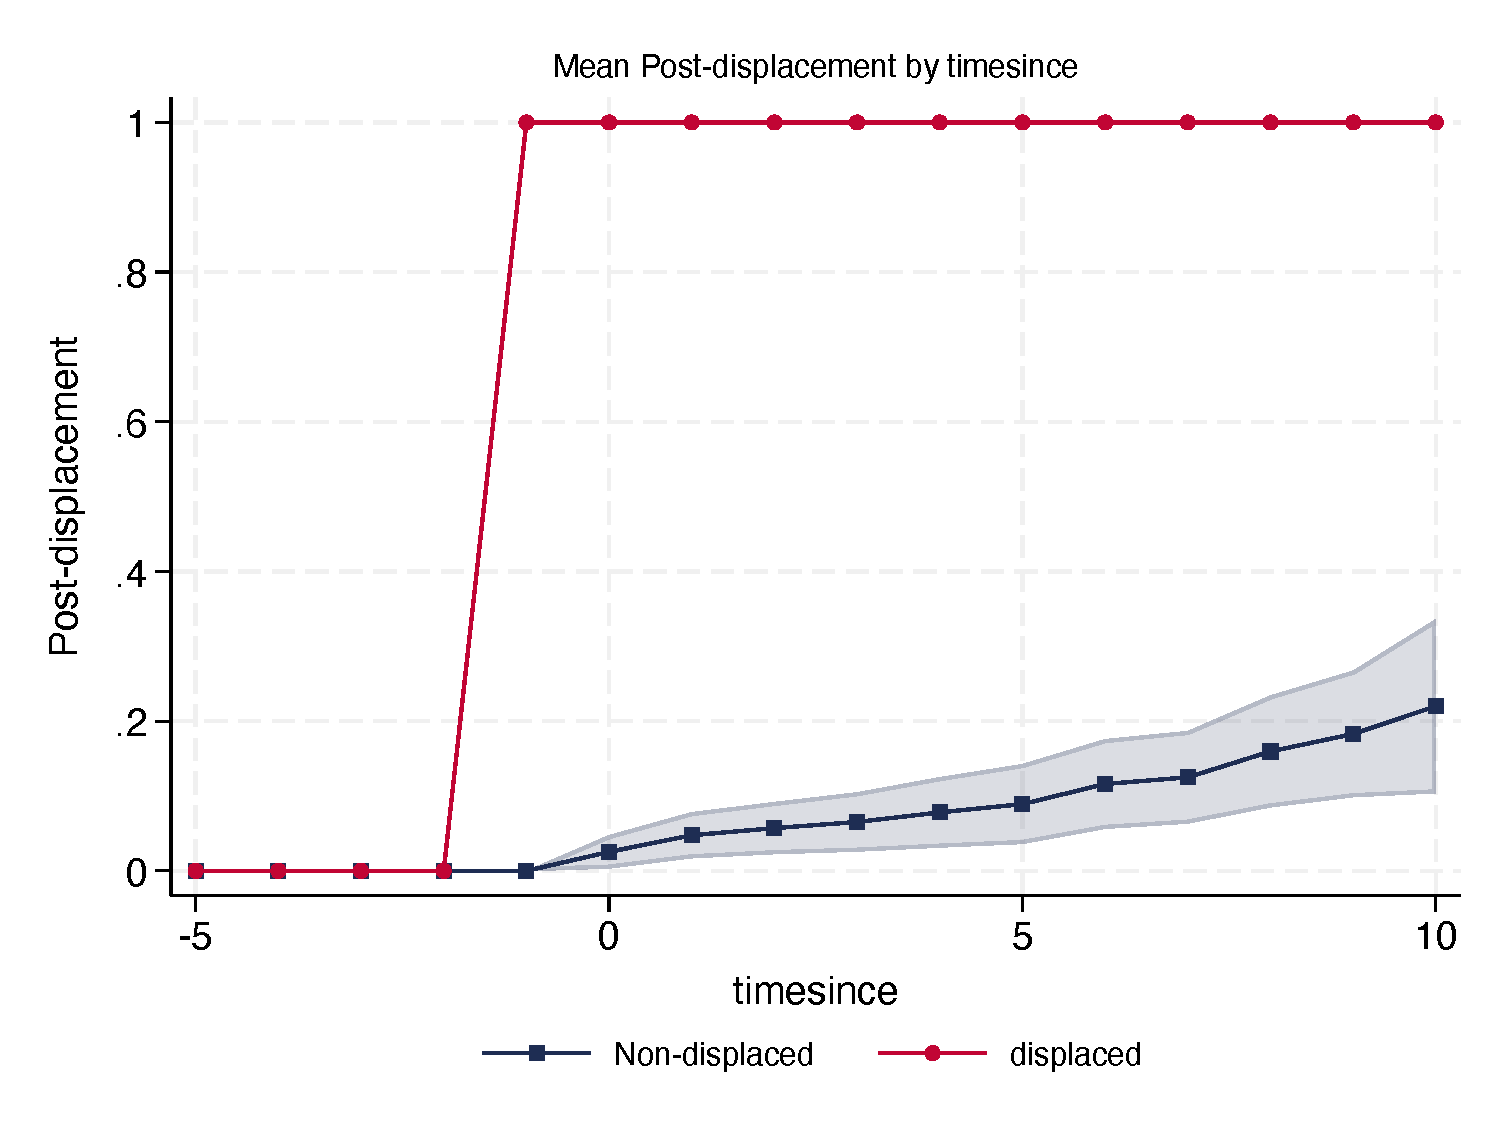
\includegraphics[width = .9\textwidth]{Disp_event_raw/displaced_by_timesince.pdf} \\ 

\end{document}
